\section{Domain adaptation}
\subsection{Overview}
So far, all approaches introduced are based on an assumption tha both training data and testing data in recognition come from the same domain, namely, training data and testing data have the same or similar distribution. It works fine if there are enough lablled training data to build up a robust classifier. However, in real world, the most costing and time-consuming process is to label samples and build up training data. At the same time, because of some reasons, there are lots of labelled samples from other domains. For example, here is a task to recognize images from Instagram, and only few images are labelled. With such a small portion of labelled images, it is difficult to build a robust classifier. However, there are thousands of labelled images which could be retrieved through search engines like Google and Bing. Once certain keywords are input to the search engines, lots of relevant images will appear, and the keywords could be used as labels of these retrieved images. Due to the differences in distribution, classifiers built from other domains work poorly in the current domain. But is it possible to utilize these labelled samples from other domains to boost the performance of classifier in the current domain? To address this problem, many domain adaptation methods \cite{daume2007frustratingly, yang2007cross, duan2009domain, duan2012visual}, which utilizes training data from other domains, have been proposed for different proposes, and these methods have been proved to be effective to build robust classifiers with few labelled samples from the target domain. \\


\begin{figure}[!ht]
\centering
  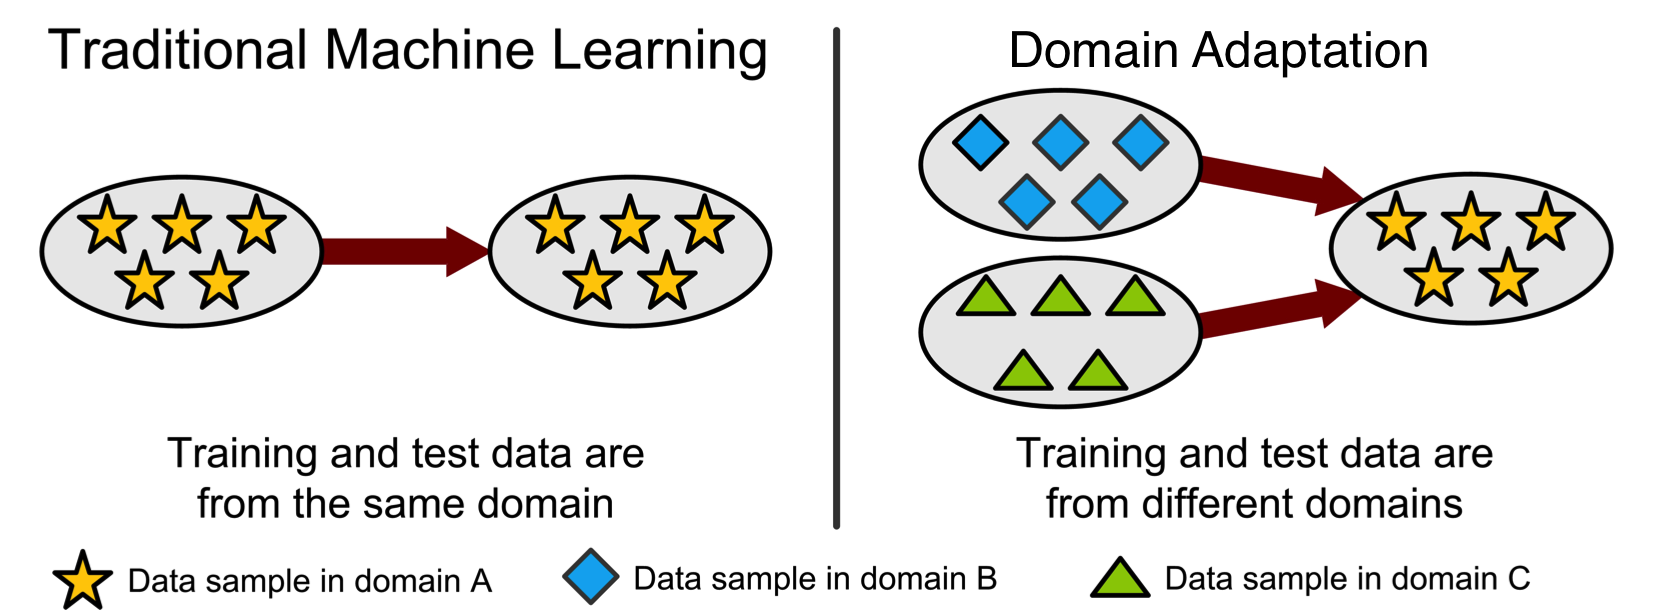
\includegraphics[width=1\textwidth]{./domainAdaption.png}
\caption{Comparison between traditional machine learning and domain adaptation. Data samples from other domains are also used as training data.}
\end{figure}

\noindent As shown in Figure 12, training data and testing data are supposed to come from the same domain in traditional machine learning. In contrast, domain adaptation also utilizes data samples from other domains. Following the terminology from literatures, the target domain, from which the test samples are, is defined as $\mathcal{D}^T$. The other domain, which provides enough labelled data, is defined as auxiliary domain $\mathcal{D}^A$. Moreover, $\mathcal{D}^T = \mathcal{D}_l^T \cup \mathcal{D}_u^T$, where $\mathcal{D}_l^T$ represents limited labelled data, and $\mathcal{D}_u^T$ represents unlabelled data. Also, the auxiliary data set $\mathcal{D}^A = \{(x_i^A, y_i^A)\}_{i=1}^{n_A}$, which is a fully labelled data set. In the rest of this section, domain adaptation methods including Feature Replication \cite{daume2007frustratingly}, Adaptive SVM \cite{yang2007cross}, Domain Transfer SVM \cite{duan2009domain} and Adaptive Multiple Kernel Learning \cite{duan2012visual} are introduced. Experimental results and analysis of these methods are presented in the section of experiments.

\subsection{Feature replication (FR)}
Feature replication \cite{daume2007frustratingly} uses augmenting features to perform SVM training. There are two different mapping functions to augment samples $\{x\}$ from different domains. 
\begin{equation}
\Phi^T(\mathbf{x}) = (\mathbf{x},\mathbf{x},\mathbf{0}), \quad  \Phi^A(\mathbf{x}) = (\mathbf{x},\mathbf{0}, \mathbf{x})
\end{equation}
where $\Phi^T$ augments samples from $\mathcal{D}^T$, and $\Phi^A$ augments samples from $\mathcal{D}^A$. The kernelized version of the above transformation is pretty straightforward. Suppose the kernel used in SVM projects sample $x$ into higher space through $\theta(x)$. Thus the kernel between $x_i$ and $x_j$ is: $K(x_i, x_j) = \theta(x_i)^T \cdot \theta(x_j)$. After the above augmenting process, 
\begin{eqnarray}
& \Phi_{\theta}^T(x) = (\theta(x), \theta(x), 0) \nonumber \\
& \Phi_{\theta}^A(x) = (\theta(x), 0, \theta(x)) 
\end{eqnarray}
where $\Phi_{\theta}^T(x)$ represents $x$ from $\mathcal{D}^T$ in higher dimensional space, and $\Phi_{\theta}^A(x)$ represents $x$ from $\mathcal{D}^A$ in higher dimensional space. The expanded kernel is defined as $\hat K(x_i, x_j)$. If $x_i$ and $x_j$ come from the same domain, 
\begin{eqnarray}
\hat K(x_i, x_j) &  = & \theta(x_i)^T \cdot \theta(x_j) + \theta(x_i)^T \cdot \theta(x_j) \nonumber \\
 & = & 2 \cdot \theta(x_i)^T \cdot \theta(x_j)   \nonumber \\
 & = & 2 K(x_i, x_j)
\end{eqnarray}
\noindent If  $x_i$ and $x_j$ come from different domains,
\begin{eqnarray}
\hat K(x_i, x_j)  & = &  \theta(x_i)^T \cdot \theta(x_j)  \nonumber \\
 & = &  K(x_i, x_j) 
\end{eqnarray}
\noindent To summarize,  
\[
 \hat K(x_i, x_j) =
  \begin{cases}
   2 K(x_i, x_j) & \text{if } x_i \text{ and } x_j \text{ come from the same domain}\\
   K(x_i, x_j)   & \text{otherwise} 
  \end{cases}
\]
\noindent Based on equations (30) and (31), considering the kernel as a measure of ``similarity'', samples from the same domain are twice as similar as those come from different domains. In order words, for a test sample, those training samples from the same domain  are going to be more influential. Furthermore, the implementation is rather easy since the only operation needed is to twice the kernels of samples from the same domain. 

\subsection{Adaptive support vector machine (A-SVM)}
Adaptive SVM \cite{yang2007cross} incorporates multiple auxiliary classifiers $f_1^A(x), \cdots, f_M^A(x)$ built from $\mathcal{D}^A$ into the standard structure of SVM. The decision function of adapted classifier is defined as
\begin{equation}
f(x) = \sum_{k=1}^M t_k f_{k}^A(x) + \Delta f(x)
\end{equation}
where $\Delta f(x) = w^T \phi(x)$ is called as a {\em permutation function} which is learned from labelled data in the target domain ($\mathcal{D}_l^T$) only, $t_k \in (0, 1)$ is the weight of each auxiliary classifier which sums to one. Because of the change in decision function, the objective function of SVM is changed to be
  \begin{eqnarray}
  & \text{minimize} \quad J(w) = \frac{1}{2} \norm{w}^2 + C \sum_{i=1}^{N}\xi_i  \nonumber \\
  & \text{subject to} \quad \xi_i \ge 0, \quad y_i \sum_{k=1}^M t_k f_{k}^A(x_i) + y_i w^{T} \phi(x_i) \ge 1 - \xi_i \quad \forall i
  \end{eqnarray}
 From the objective function listed above, it is not hard to distinguish that Adaptive SVM aims to find a hyperplane which is not only close to hyperplanes built from $\mathcal{D}^A$ but also separates labelled samples in $\mathcal{D}^T$ well. Due the change of objective function, the Lagrange dual form is changed to be 
  \begin{equation}
  W(\alpha) = \sum_{i} (1 - \lambda_i) \alpha_i - \frac{1}{2} \sum_{i,j} y_i y_j \alpha_i \alpha_j K(x_i, x_j)
  \end{equation}
  where $\lambda_i = y_i \sum_{k=1}^M t_k f_{k}^A(x_i)$. Once the set $\hat \alpha$ which maximizes $W(\alpha)$ is found, the decision function $f(x)$ is expressed as 
 \begin{equation}
f(x) = \sum_{k=1}^M t_k f_{k}^A(x) + \sum_i \hat \alpha_i y_i K(x_i, x)
\end{equation}

\subsection{Domain transfer support vector machine (DTSVM)}
It has been emphasized that the distributions of $\mathcal{D}^T$ and $\mathcal{D}^A$ are different. Therefore, when these two sets of data are projected into higher dimensional space, their distributions are still distant to each other. If there is a way to reduce the mismatch between $\mathcal{D}^T$ and $\mathcal{D}^A$, then those lablled samples from $\mathcal{D}^A$ could be treated as samples in the target domain to some extent, and of course this is going to improve the performance of recognition because more useful training samples are input to build a robust classifier. Given the fact that fusing multiple kernels helps to increase the performance, Duan et al. \cite{duan2009domain} proposed Domain Transfer SVM (DTSVM) to reduce the mismatch between $\mathcal{D}^T$ and $\mathcal{D}^A$ through calculating the optimal weight of each kernel. Also, the respective classifier is learnt simultaneously. \\

\noindent The mismatch measured by Maximum Mean Discrepancy (MMD) \cite{borgwardt2006integrating} is defined as follows
\begin{equation}
DIST_k(\mathcal{D}^A, \mathcal{D}^T) = \norm{\frac{1}{n_A} \sum_{i=1}^{n_A} \varphi(x_i^A) - \frac{1}{n_T} \sum_{i=1}^{n_T} \varphi{x_i^T}}
\end{equation}
where $x_i^A$ and $x_i^T$ are samples from the auxiliary and target domains, respectively, and $\varphi(x)$ is a mapping function which projects $x$ into higher dimensional space. Given this mapping function, the kernel between $x_i$
 and $x_j$ is $k(x_i, x_j) = \varphi (x_i)^T \cdot \varphi (x_j)$. To simplify equation (36), a column vector $\mathbf{s}$, in which the first $n_A$ entries are $\frac{1}{n_A}$ while the remaining $n_T$ entries are $-\frac{1}{n_T}$. Now the square of MMD in equation (36) is simplified as 
\begin{equation}
DIST_k^2(\mathcal{D}^A, \mathcal{D}^T) = \text{tr}(\mathbf{KS})
\end{equation}
where $\mathbf{S = s s^T }$, and $\mathbf{K = \begin{bmatrix} K^{A,A} & K^{A,T} \\ K^{T, A} & K^{T,T}\\  \end{bmatrix}}$, and $K^{A,A}$, $K^{T,T}$ and $K^{A, T}$ are kernel matrices defined for auxiliary domain, target domain and the cross domain for the auxiliary domain to target domain.\\ 

\noindent According to traditional multiple kernel learning assumptin \cite{lanckriet2004learning}, the final kernel $k$ is a result of linear combination of several base kernels $k_1, \cdots, k_M$.
\begin{equation}
k = \sum_{m=1}^{M}d_m k_m
\end{equation}
where $d_m$ is the coefficient of $k_m$ with constraints $d_m \geq 0$ and $\sum_{i=1}^{M}d_m = 1$. Based on final kernel $k$, the decision function is thus defined as
\begin{equation}
f^T(x) = \sum_{m=1}^{M} d_m w_m^T \varphi_m(x) + b 
\end{equation}
where $f^T(x)$ is the permutation function built by $\mathcal{D}_l^T$ based on base kernels with $b$ as the bias term. As a result, once the optimal coefficients $\mathbf{d}=[d_1, \cdots, d_M]^T$ are found through the process of reducing mismatches between $\mathcal{D}^T$ and $\mathcal{D}^A$, this decision function will be easily defined. After incorporating equation (38) into (37), the square of MMD is defined as a function of $\mathbf{d}$.
\begin{equation}
DIST_k^2(\mathcal{D}^A, \mathcal{D}^T) = \Omega(\mathbf{d}) = \mathbf{h^T d}
\end{equation}
where $\mathbf{h} = [tr(\mathbf{K_1 S}), \cdots, tr(\mathbf{K_MS})]^T$, and $\mathbf{K_m} = [\varphi(x)^T \varphi(x)]$ is the $m$th base kernel matrix defined on samples from both auxiliary and target domains. After all these settings, the optimization problem of DTSVM is defined as 
\begin{equation}
\text{minimize} \quad G(\mathbf{d}) = \frac{1}{2} \Omega^2(\mathbf{d}) + \theta J(\mathbf{d})
\end{equation}
where $\theta$ is is a tradeoff parameter which balances the mismatch of distributions and the structural risk function of SVM, and 
  \begin{equation}
  J(\mathbf{d}) = \underset{\boldsymbol{\alpha}}{\max} \; \sum_i \alpha_i - \frac{1}{2} \sum_{i,j} y_i y_j \alpha_i \alpha_j  (\sum_{m=1}^M d_m \; \varphi_m (x_i) ^T \varphi_m (x_j))           
  \end{equation}
To solve the optimization problem, the author \cite{duan2009domain} employed the reduced gradient descent procedure to iteratively update coefficients $\mathbf{d}$ and dual variable $\boldsymbol{\alpha}$. There are two steps:
\begin{enumerate}
	\item{\bf Update the dual variable $\boldsymbol{\alpha}$} \\
	Given the current value $\mathbf{d}$, the optimization problem in equation (42) are  solved by LIBSVM \cite{CC01a}, and the dual variable $\boldsymbol{\alpha}$ is updated.

	\item{\bf Update the linear combination coefficients $\mathbf{d}$}\\
	At $ t+1 $ iteration, $d_{t+1}$ is updated as
	\begin{equation}
	\mathbf{d}_{t+1} = (1 - \eta_t) \mathbf{d}_{t} + \eta_t \mathbf{d}_t^{new}
	\end{equation}
	where $\mathbf{d}_t^{new} = \theta(\mathbf{h h^T} + \varepsilon \mathbf{I_M})^{-1} \mathbf{q}$, and $\varepsilon \mathbf{I_M}^{-1}$ is added to avoid numerical instability with $\varepsilon = 10^{-5}$, and $\mathbf{q} = [\frac{1}{2}(\boldsymbol{\alpha}_t \diamond \mathbf{y})^T \mathbf{K}_1 (\boldsymbol{\alpha}_t \diamond \mathbf{y}), \cdots, \frac{1}{2}(\boldsymbol{\alpha}_t \diamond \mathbf{y})^T \mathbf{K}_M (\boldsymbol{\alpha}_t \diamond \mathbf{y})]$, and $\eta_t$ is the learning rate. Please note the symbol $\diamond$ represents the element-wise product of two vectors. For formal mathematical induction, please refer to \cite{duan2009domain,duan2012visual} for details, and a formal and concise algorithm description is presented in \cite{duan2012visual}. 
\end{enumerate}

\noindent The above two steps are repeated until convergence or the maximum number of iteration allowed is reached. At the end of this algorithm, the optimal $\mathbf{d}$ is learned as well as the optimal SVM model.

\noindent 
\subsection{Adaptive multiple kernel learning (A-MKL)}
Inspired by adaptive SVM (A-SVM) \cite{yang2007cross} and domain transfer SVM (DTSVM) \cite{duan2009domain}, the authors of DTSVM creatively combined these two approaches and proposed adaptive multiple kernel learning (A-MKL) \cite{duan2012visual}.  A-MKL takes the advantage of pre-learnt classifiers built either from $\mathcal{D}^A$ or $\mathcal{D}^A \cup \mathcal{D}^T$ and defines the decision function as
\begin{equation}
f^T(x) = \sum_{p=1}^{P} \beta_p f_p(x) + \sum_{m=1}^{M} d_m w_m^T \varphi_m(x) + b 
\end{equation}
Compared with equation (39), the added item $\sum_{p=1}^{P} \beta_p f_p(x)$, where $f_1(x), \cdots, f_P(x)$ are pre-learnt classifiers with $\beta$ being the weight of each classifier, represents the influence from pre-learnt classifiers. Because of the influence coming from pre-learnt classifiers, compared with DTSVM, the difference is that equation (42) becomes
\begin{equation}
J(\mathbf{d}) = \underset{\boldsymbol{\alpha}}{\max} \; \sum_i \alpha_i - \frac{1}{2} \sum_{i,j} y_i y_j \alpha_i \alpha_j  (\sum_{m=1}^M d_m \; \breve{\varphi_m} (x_i) ^T \breve{\varphi_m} (x_j))           
\end{equation}
where $\breve{\varphi_m} (x_i) ^T \breve{\varphi_m} (x_j) = \varphi_m (x_i) ^T \varphi_m (x_j) + \frac{1}{\lambda} \boldsymbol{f} (x_i)^T \boldsymbol{f}  (x_j)$, and $\boldsymbol{f}(x)$ is a vector of predictions on $x$ from pre-learnt classifiers $f_1(x), \cdots, f_P(x)$, and $\lambda$ is a regularization parameter in the objective function of SVM. Since the only change is the kernel matrix, once the kernel matrix is fused by scores of pre-learnt classifiers, the algorithm used in DTSVM could be directly employed to calculate the optimal coefficients $\mathbf{d}$ and dual variables $\boldsymbol{\alpha}$. With the help from scores output by pre-learnt classifiers, A-MKL not only reduces the mismatch of distributions between $\mathcal{D}^A$ and $\mathcal{D}^T$ but also finds a hyperplane which is close to the optimal hyperplane of $\mathcal{D}^A$ in ``new'' distribution. 
